\documentclass{article}
\setlength\parindent{0pt}



\usepackage {graphicx} % Required for inserting images
\usepackage{pgfplots}
\pgfplotsset{compat=1.18}
\usepackage{amsmath}
\usepackage{amssymb}
\usepackage{wrapfig}
\usepackage{ragged2e}
\usepackage{hyperref}
\usepackage[many]{tcolorbox}
\usepackage{amsthm}
\tcbuselibrary{theorems}
\usepackage{bm}
\usepackage{subcaption}
\usepackage{mathtools}


\theoremstyle{definition}
\newtheorem{exmp}{Example}[section]

\DeclarePairedDelimiter{\abs}{\lvert}{\rvert}
\DeclarePairedDelimiter{\curly}{\{}{\}}

\newtcbtheorem[number within=section]{theorem}{Theorem}%
{colback=blue!5,colframe=blue!35!black,fonttitle=\bfseries}{th}

\newtcbtheorem[number within=section]{definition}{Definition}%
{colback=red!5,colframe=red!35!black,fonttitle=\bfseries}{th}


\definecolor{greentitle}{RGB}{61,170,61}
\definecolor{greentitleback}{RGB}{216,233,213}

\newtcolorbox[
  auto counter,
  number within=section
]{myexample}[2][]{%
  breakable,
  enhanced,
  colback=white,
  colbacktitle=white,
  arc=0pt,
  leftrule=1pt,
  rightrule=0pt,
  toprule=0pt,
  bottomrule=0pt,
  titlerule=0pt,
  colframe=greentitleback,
  fonttitle=\normalcolor,
  overlay={
    \node[
      outer sep=0pt,
      anchor=east,
      text width=2.5cm,
      minimum height=4ex,
      fill=greentitleback,
      font=\color{greentitle}\sffamily\scshape
    ] at (title.west) {example~\thetcbcounter};
  },
  title=#2,
  #1
}
\newcommand\Solution{\par\textbf{\textsf{Solution}}\par\medskip}





\title{Chapter 9 Notes}
\author{Pranaav Sureshkumar}

\begin{document}

\maketitle

\tableofcontents

\section*{Conventions}
To establish a consistent naming convention; in these notes $\mathbb{R}$ is the set of all real numbers ($-7, -2.5, \pi, 14,\cdots$), $\mathbb{Z}$ is the set of all integers ($-2,-1,0,1,\cdots$), $\mathbb{N}$ is the set of all natural numbers ($0,1,2,\cdots$), and $\mathbb{Z_+}$ is the set of all strictly positive integers ($1,2,3,\cdots$). Often, sigma notation ($\sum$) will be used without specifying an index to represent generic series in which the starting index is insignificant.


\section{Day 1 | 9.1 Sequences \& Factorials}

\vspace{0.5cm}

\subsection{Sequences}
A sequence is a discrete function that maps a non-negative integer, typically denoted $n$, to a corresponding value in a set of numbers.
Consider the sequences:



\[a_n  = 2n-5 \text{ whose first five terms are } \curly*{-3, -1, 1, 3, 5}.\]
\begin{center}
    Since $\displaystyle\lim_{n \to \infty} a_n =\infty$, $a_n$ diverges.
\end{center}

\[a_n  = \frac{1}{2^n} \text{ whose first five terms are } \curly*{\frac{1}{2}, \frac{1}{4}, \frac{1}{8}, \frac{1}{16}, \frac{1}{32}}.\]

\begin{center}
    Since $\displaystyle\lim_{n \to \infty} a_n = 0$, $a_n$ converges to 0.
\end{center}

\[a_n  = \frac{(-1)^{n+1}}{n} \text{ whose first five terms are } \curly*{1, -\frac{1}{2}, \frac{1}{3}, -\frac{1}{4}, \frac{1}{5}}.\]

\begin{center}
    Since $\displaystyle\lim_{n \to \infty} a_n = 0$, $a_n$ converges to 0.
\end{center}

\[a_n  = \frac{5n+1}{2n} \text{ whose first five terms are } \curly*{3, \frac{11}{4}, \frac{8}{3}, \frac{21}{8}, \frac{13}{5}}.\]

\begin{center}
    Since $\displaystyle\lim_{n \to \infty} a_n = \frac{5}{2}$, $a_n$ converges to $\frac{5}{2}$.
\end{center}

\[a_n  = 3+(-1)^n \text{ whose first five terms are } \curly*{2, 4, 2, 4, 2}.\]

\begin{center}
    Since $\displaystyle\lim_{n \to \infty} a_n$ does not exist, $a_n$ diverges.
\end{center}

\vspace{0.5cm}

\begin{definition}{Convergence \& Divergence of Sequences}{Sequences}
\vspace{-0.5cm}
    \[ \text{ If } \lim_{n \to \infty} a_n = c \text{ where } c \text{ is finite and positive, then } a_n \text{ converges to } c. \]
    \vspace{-0.5cm}
    \[ \text{ If } \lim_{n \to \infty} a_n \text{ does not exist or equals $\pm \infty$, then } a_n \text{ diverges.}\]
\end{definition}

A series is the sum of the terms in a sequence. The sum of the first $k$ terms of a sequence $a_n$ is symbolically represented with sigma notation as \[\sum_{n=1}^{k} a_n.\]

\subsection{Factorials}

The factorial is a function defined on the input set $x \in \mathbb{N}$ that multiplies an input by every consecutive decreasing integer value, until 1.

\begin{definition}{Factorial}{Factorials}

\[n!=n\times(n-1)\times(n-2)\times \cdots \times 1\]
\end{definition}

\[\frac{10!}{7!} \text{ can be simplified to } \frac{10 \cdot 9 \cdot 8 \cdot 7!}{7!}=10\cdot9\cdot8=720.\]

\begin{center}
    $0!=1$ is a special factorial case.
\end{center}



\section{Day 2 | 9.2 Series \& Convergence}

\subsection{Geometric Series}
A geometric sequence has a first term and a common ratio by which each subsequent term is multiplied. A geometric sequence where $a$ is the first term and $r$ is the common ratio has terms $\curly{a, ar, ar^2, ar^3, ar^4, \cdots}$.
An infinite geometric series \textbf{converges} if $\lvert r \rvert <1$ and \textbf{diverges} otherwise.


\[\text{Consider: the infinite geometric series } \sum_{n=0}^{\infty} ar^n \text{ where } \lim_{n \to \infty} a_n=0.\]

\[\text{Let $S$ represent the value of the series.}\]
\[S=ar^0+ar^1+ar^2+ar^3+\cdots\]

\[S=r(ar^{-1}+\underbrace{ar^0+ar^1+ar^2+ar^3+\cdots}_ {S})\] \marginpar{For fun, try factoring $r^2$ instead of $r$ and continue with the proof.}

\[S=r(ar^{-1}+S)\]

\[S=a+rS\]

\[S-rS=a\]

\[(1-r)S=a\]

\[S=\frac{a}{1-r}.\]

\begin{theorem}{Value of an Infinite Geometric Series}{Geometric Series}
\vspace{-0.3cm}
    \[\text{If an infinite geometric series converges ($\abs{r}<1$), then it does so to } \frac{a}{1-r}.\]
\end{theorem}

\subsection{$n$\textsuperscript{th} Term Test}
If a sequence does not converge to 0, its series \textbf{cannot} converge because any nonzero number, no matter how small, diverges to $\pm \infty$ when added infinitely. However, the inverse statement is not necessarily true as a sequence that converges to 0 can still have a series that diverges. (consider $a_n=\frac{1}{x}$)

\[\text{Consider: } \sum_{n=1}^{\infty} \frac{n^2}{3n^2+1}=\frac{1}{4}+\frac{4}{13}+\frac{9}{28}+\frac{16}{49}+\cdots + \underbrace{\frac{1}{3}+\frac{1}{3}+\frac{1}{3}}_{\infty \text{ times}}.\]
\[\text{Therefore, } \sum_{n=1}^{\infty} \frac{n^2}{3n^2+1} \text{ diverges.}\]

\begin{theorem}{$n$\textsuperscript{th} Term Test}{nth Term Test}
    \[\text{If } \lim_{n \to \infty} a_n \not= 0 \text{, then } \sum^{\infty} a_n \textbf{ diverges.}\]
    \[\text{If } \lim_{n \to \infty} a_n     = 0 \text{, then no definitive conclusion can be drawn.}\]
\end{theorem}

\subsection{Telescoping Series}
Telescoping series are referred to as such because they expand infinitely and cancel to a finite value.




\[\text{Consider: } S_\infty=\sum_{n=1}^{\infty} \frac{1}{n^2+3n+2}.\]

\[S_\infty = \sum_{n=1}^{\infty} \frac{1}{n^2+3n+2} = \sum_{n=1}^{\infty} \frac{1}{(n+2)(n+1)}=\underbrace{\sum_{n=1}^{\infty} \frac{1}{n+1}-\frac{1}{n+2}}_{\text{by partial fraction decomposition}}\]


\newpage

\[\text{Generating terms:}\]

\begin{equation*}
\begin{split}
    S_1&=\frac{1}{2}-\frac{1}{3} \\
    S_2&=\frac{1}{2}-\frac{1}{3}+\frac{1}{3}-\frac{1}{4} \\
    S_3&=\frac{1}{2}-\frac{1}{3}+\frac{1}{3}-\frac{1}{4}+\frac{1}{4}-\frac{1}{5} \\
    S_4&=\frac{1}{2}-\frac{1}{3}+\frac{1}{3}-\frac{1}{4}+\frac{1}{4}-\frac{1}{5}+\frac{1}{5}-\frac{1}{6}
\end{split}
\end{equation*}

Following $\frac{1}{2}$, all terms cancel with subsequent terms---the defining characteristic of a telescoping series. Therefore, $S_\infty$ converges to $\frac{1}{2}$.



\section{Day 3 | 9.3 Integral Test}
The integral test works by using an integral to approximate the value of a monotone decreasing series. If an integral converges, the infinite series it represents converges as well. If an integral diverges, the infinite series it represents must also diverge. The integral test is requisite to determine that harmonic series diverge.

\begin{theorem}{The Integral Test}{Integral Test}
    If $f$ is a function that is positive, continuous, and \textbf{monotone decreasing} over $[c, \infty]$ such that $f(n)= a_n$, then
    \vspace{-0.3cm}
    \[\int_{c}^{\infty}f(x)dx \text{ and } \sum_{n=c}^{\infty} a_n \text{ behave the same way.}\]
\end{theorem}

\[\text{Consider: } S_\infty=\sum_{n=1}^{\infty} \frac{n}{n^2+3}. \text{ To evaluate, compare to} \int_{1}^{\infty} \frac{n}{n^2+3}.\]


\begin{align*}
\text{Using } u &= n^2 + 3 \\
\text{and } du &= 2ndn, \\
\int_{1}^{\infty} \frac{n}{n^2+3}dn &= \frac{1}{2} \int_{4}^{\infty} \frac{1}{u}du \\
&= \frac{1}{2} [\ln|u|]^{\infty}_{4}\\
&= \infty.
\end{align*}

\[\text{Therefore, $S_\infty$ diverges.}\]

\newpage

\section{Day 3 | 9.4 Comparison Tests}

\subsection{Direct Comparison Test}
The direct comparison test works by comparing an unknown series to a known series to determine the qualities of the unknown series. It relies on the principle that a series that is larger\footnote{Both series must be greater than zero, so it is not possible for a series to be \emph{more negative than} (less than) another with this test.} than a series that diverges must also diverge. The contrapositive statement is also true.

\begin{theorem}{The Direct Comparison Test}{DCT}
    For $0 \le a_n \le b_n$:
            \[\text{If } \underbrace{\sum^{\infty} b_n}_{\text{larger}} \text{ converges, then } \underbrace{\sum^{\infty} a_n}_{\text{smaller}} \text{ converges as well.}\]

            \[\text{If } \underbrace{\sum^{\infty} a_n}_{\text{smaller}} \text{ diverges, then } \underbrace{\sum^{\infty} b_n}_{\text{larger}} \text{ diverges as well.}\]

\end{theorem}


\noindent\begin{minipage}{\textwidth} % Allows for centering
\[
\hidewidth
\text{Consider: } S_\infty=\sum_{n=1}^{\infty} \frac{1}{n^3+1}. \text{ To evaluate, compare to } \sum_{n=1}^{\infty} \frac{1}{n^3} \text{ which is known to converge.}
\hidewidth
\]
\end{minipage}

\[\text{Since } \sum_{n=1}^{\infty} \frac{1}{n^3+1} \le \sum_{n=1}^{\infty} \frac{1}{n^3} \text{ and } \sum_{n=1}^{\infty} \frac{1}{n^3} \text{ converges, } \sum_{n=1}^{\infty} \frac{1}{n^3+1} \text{ converges as well.}\]

\subsection{Limit Comparison Test}
The limit comparison test is used more often than the direct comparison test and provides a more concrete result. It compares the ratio of two similar discrete functions to determine whether they behave similarly.

\begin{theorem}{The Limit Comparison Test}{LCT}
    For $a_n \ge 0$ and $b_n \ge 0$:
    
\[\text{If } \frac{a_n}{b_n}=L \text{ where $L$ is finite and \textbf{strictly positive}, then}\]
\vspace{-0.3cm}
\[\sum^{\infty} a_n \text{ and } \sum^{\infty} b_n \text{ behave the same way.}\]
    
\end{theorem}

\[\text{Consider: } \sum_{n=5}^{\infty} \frac{n^2-10}{4n^5-n^3+7}. \text{ To evaluate, compare to } \sum_{n=5}^{\infty} \frac{1}{n^3}.\]

\[\lim_{n \to \infty} \frac{\frac{n^2-10}{4n^5-n^3+7}}{\frac{1}{n^3}}\]
\[=\lim_{n \to \infty} \frac{n^5-10n^3}{4n^5-n^3+7}=\frac{1}{4}.\]

\vspace{1cm}



\section{Day 4 | 9.5 Alternating Series Test}
Alternating series have both positive and negative terms. In \emph{strictly} alternating series, positive and negative terms must be immediately adjacent.

\begin{theorem}{Alternating Series Test}{AST}
\[\sum^{\infty} (-1)^n a_n \text{ converges \textbf{only} if } a_{n+1} \le a_n \textbf{ and } \lim_{n \to \infty} a_n=0.\] 
\end{theorem}

\[\sum_{n=1}^{\infty} \frac{1}{n} \text{ is known to converge. Now consider: } S_\infty=\sum_{n=1}^{\infty} \frac{(-1)^{n+1}}{n}\]

\[\text{When expanded, } S_\infty=1-\frac{1}{2}+\frac{1}{3}-\frac{1}{4}+\frac{1}{5} \cdots \]

\[\text{First, isolate the alternator by rewriting $S_\infty$ as } \sum_{n=1}^{\infty} (-1)^{n+1}\frac{1}{n}.\]
\[\frac{1}{n+1} \le \frac{1}{n} \text{ is always true.}\]
\[\lim_{n \to \infty} \frac{1}{n}=0 \text{ is always true.}\]
\[\textbf{Therefore, $S_\infty$ converges by the AST.}\]

\vspace{0.5cm}

This alternating variant of the simple harmonic series converges, but the standard harmonic series does not. This is known as \emph{conditional convergence}.

\begin{definition}{Conditional \& Absolute Convergence}{CAC}
\vspace{-0.5cm}
    \[\text{Conditional convergence: } \sum^{\infty} (-1)^n a_n \text{ converges, but } \sum^{\infty} a_n \text{ diverges.}\]
\vspace{-0.5cm}
    \[\text{Absolute convergence: } \sum^{\infty} (-1)^n a_n \text{ converges, and } \sum^{\infty} a_n \text{ converges.}\]
\end{definition}



\section{Day 5 | 9.5 Alternating Series Error Bound}

\vspace{0.5cm}

\[\text{Consider: } S_\infty = \sum_{n=1}^{\infty} \frac{(-1)^{n+1}}{n}=1-\frac{1}{2}+\frac{1}{3}-\frac{1}{4}+\cdots\]


\[\text{The partial sums are:}\]

\[S_1=1\]
\[S_2=\frac{1}{2}\]
\[S_3=\frac{5}{6}\]
\[S_4=\frac{7}{12}\]



\begin{figure}[h]
\centering

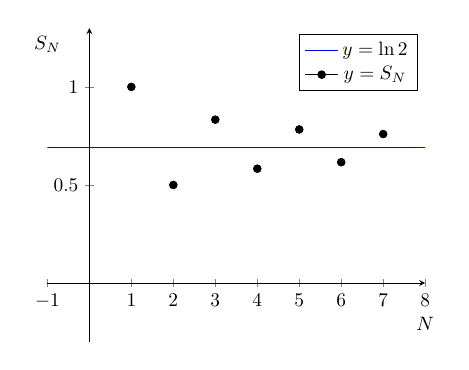
\begin{tikzpicture}[scale=0.7]
\begin{axis}[
    axis x line=middle,
    axis y line=middle,
    xmin=-1, xmax=8,
    ymin=-0.3, ymax=1.3,
    xtick distance=1,
    x label style={at={(axis description cs:1,0.1)},anchor=north},
    y label style={at={(axis description cs:0,0.9)},anchor=south},
    xlabel=$N$,
    ylabel=$S_N$
]
    \addplot[blue, domain=-1:9, samples=100] {0.69314718056};
    \addlegendentry{$y = \ln{2}$}
    \addplot[mark=*] coordinates {(1,1)};
    \addplot[mark=*] coordinates {(2,0.5)};
    \addplot[mark=*] coordinates {(3,0.833)};
    \addplot[mark=*] coordinates {(4,0.583)};
    \addplot[mark=*] coordinates {(5,0.783)};
    \addplot[mark=*] coordinates {(6,0.616)};
    \addplot[mark=*] coordinates {(7,0.759523809523)};
    \addlegendentry{$y = S_N$};
    
    


\end{axis}
\end{tikzpicture}

\caption{Graph of $S_N$ with respect to $N$}
\end{figure}

\[\sum_{n=1}^{\infty} \frac{(-1)^{n+1}}{n} \text{ converges to } \ln 2.\]

\vspace{0.5cm}

\begin{theorem}{Error Bound}{1}
The sum of a convergent, \emph{strictly}\footnote[1]{If $S_4=1+2-3-4 \text{, $S$ is \textbf{not} strictly alternating.}$} alternating series of infinite terms $S_\infty$ will differ from the partial sum of $N$ terms $S_N$ by no more than the value of the \textbf{first omitted term} ($a_{N+1}$).
\end{theorem}

\vspace{0.5cm}

Problems you could be given include:
\begin{itemize}
    \item Approximate the infinite sum using $N$ terms.
    \item Determine the error bound for a partial sum of $N$ terms.
    \item Determine the number of terms required to approximate the infinite sum within (some given error) (ex. error less than $\frac{1}{10}$). The first term less than $\frac{1}{10}$ is $\frac{1}{11}$. 
    \vspace{0.1cm}
    Therefore, ten terms are required for the error bound to be less than $\frac{1}{10}$.
    \item Which term represents (some given error bound)?
\end{itemize}

\vspace{0.5 cm}


\[ \textbf{Consider: } \sum_{n=0}^{\infty} \frac{(-1)^n}{(2n+1)!}.\] 
\[\text{First, perform a simple AST test. Is } a_{n+1}<a_n?\]
\[\frac{1}{(2n+3)!}<\frac{1}{(2n+1)!} \text{ is true.}\]

\[\text{Then, generate terms.}\]


\[\frac{1}{1!} - \frac{1}{3!} + \frac{1}{5!} - \frac{1}{7!} + \cdots\]

\[\text{Compute partial sums.}\]

\[S_2=\frac{5}{6} \text{ whose error bound is } \frac{1}{5!}=\frac{1}{120}.\]
\[S_3=\frac{101}{120} \text{ whose error bound is } \frac{1}{7!}=\frac{1}{5040}.\]

\vspace{1cm}

\[\sum_{n=0}^{\infty} \frac{(-1)^n}{(2n+1)!} \text{ converges to } \sin 1.\]



\section{Day 6 | 9.6 Ratio Test \& $n$\textsuperscript{th} Root Test}
\vspace{0.3cm}
\subsection{Ratio Test}
If every term in a sequence is less than its preceding term (the sequence is decreasing quickly), then its series must converge. The inverse statement is also true. 

\begin{theorem}{Ratio Test}{2}

\[\sum^{\infty} a_n \text{ \textbf{converges} absolutely if } \lim_{n \to \infty} \abs*{\frac{a_{n+1}}{a_n}} < 1\]

\[\sum^{\infty} a_n \text{ \textbf{diverges} absolutely  if } \lim_{n \to \infty} \abs*{ \frac{a_{n+1}}{a_n}} > 1\]

\[\sum^{\infty} a_n \text{ is \textbf{inconclusive} if } \lim_{n \to \infty} \abs*{\frac{a_{n+1}}{a_n}} = 1\]

\end{theorem}

\vspace{0.5 cm}

\[ \textbf{Determine if } \sum_{n=0}^{\infty} \frac{2^n}{n!} \text{ converges.}\]

\[\text{Ratio test:}
  \lim_{n \to \infty} \abs*{\frac{\frac{2^{n+1}}{(n+1)!}}{\frac{2^n}{n!}}}
= \lim_{n \to \infty} \abs*{\frac{2^{n+1}}{(n+1)!}  \cdot {\frac{n!}{2^n}}}
= \lim_{n \to \infty} \abs*{\frac{2}{n+1}} = 0 < 1 \]

\[\text{Therefore, }\sum_{n=0}^{\infty} \frac{2^n}{n!} \text{ converges.}\]

\vspace{0.5cm}

\[ \textbf{Determine if } \sum_{n=0}^{\infty} \frac{(-1)^n \cdot n^3 \cdot 2^{n+2}}{3^n} \text{ converges.} \]
\[ \textbf{Let } S_\infty=\sum_{n=0}^{\infty} \frac{(-1)^n \cdot n^3 \cdot 2^{n+2}}{3^n}\]


\[\text{Ratio test: } \lim_{n \to \infty} \abs*{\frac{(-1)^{n+1} \cdot (n+1)^3 \cdot 2^{n+3}}{3^{n+1}} \cdot \frac{3^n}{(-1)^n \cdot n^3 \cdot 2^{n+1}}} = \frac{2}{3} < 1\]

\[\text{Therefore, }\sum_{n=0}^{\infty} \frac{(-1)^n \cdot n^3 \cdot 2^{n+2}}{3^n} \text{ converges.}\]


\vspace{0.5cm}

\[ \textbf{Determine if } \sum_{n=1}^{\infty} \frac{n^n}{n!} \text{ converges.} \]
\[ \textbf{Let } S_\infty=\sum_{n=1}^{\infty} \frac{n^n}{n!}\]

\[\text{Ratio test: }\lim_{n \to \infty} \abs*{  \frac{(n+1)^{n+1}}{(n+1)!} \cdot \frac{n!}{n^n}}
= \lim_{n \to \infty} \abs*{ \frac{(n+1)^n}{n^n}} = \lim_{n \to \infty} \abs*{(1+\frac{1}{n})^n} = e > 1\]

\[\text{Therefore, }\sum_{n=1}^{\infty} \frac{n^n}{n!} \text{ converges.}\]




\subsection{$n$\textsuperscript{th} Root Test}

\[\text{Let } \sqrt[n]{\abs{a_n}} \le k < 1.\]
\[\text{Then, } \abs{a_n} \le k^n < 1.\]
By the direct comparison test,  since $\sum^{\infty}k^n \text{ converges when } k<1$, $\sqrt[n]{\abs{a_n}}$ also converges.

\begin{theorem}{$n$\textsuperscript{th} Root Test}{3}
\[\text{If } \lim_{n \to \infty} \sqrt[n]{\abs*{a_n}} < 1 \text{, then } a_n \text{ converges absolutely.} \]

\[\text{If } \lim_{n \to \infty} \sqrt[n]{\abs*{a_n}} > 1 \text{, then } a_n \text{ diverges absolutely.} \]

\[\text{If } \lim_{n \to \infty} \sqrt[n]{\abs*{a_n}} = 1 \text{, then the test is inconclusive.}\]
\end{theorem}

\[\text{Determine if }\sum_{n=1}^{\infty} \frac{e^{2n}}{n^n}\text{converges.}\]


\[\text{Using the $n$\textsuperscript{th} root test, }\lim_{n \to \infty} \sqrt[n]{\frac{e^{2n}}{n^n}} = \lim_{n \to \infty} \frac{e^2}{n} = 0 < 1\]

\[\text{Therefore, }\sum_{n=1}^{\infty} \frac{e^{2n}}{n^n} \text{ converges.}\]

\newpage

\section{Day 1 | 9.7 Taylor Polynomials}

Polynomial functions are often more cooperative and nicer to deal with than non-polynomial functions. Taylor Polynomials\footnote{\textit{Taylor Polynomials} are partial sums of \textit{Taylor Series}.} allow for approximating non-polynomial functions with polynomial functions.

\vspace{0.5cm}

Consider the generic fifth-degree polynomial $P(x)=a_0 + a_1x + a_2x^2 + a_3x^3 + a_4x^4 + a_5x^5$ where $a_n$ represents the coefficient of the $n$\textsuperscript{th} power of $x$.

\begin{equation*}
\begin{split}
    f'(x)&= a_1 + 2a_2x + 3a_3x^2 + 4a_4x^3 + 5a_5x^4\\
    f''(x)&=2a_2 + 6a_3x + 12a_4x^2 + 20a_5x^3\\
    f'''(x)&=6a_3 + 24a_4x + 60a_5x^2\\
    f^{(4)}(x)&=24a_4 + 120a_5x\\
    f^{(5)}(x)&=120a_5
\end{split}
\end{equation*}

\vspace{0.5cm}
To construct a polynomial function $P$ such that $P(0)=10$, $P'(0)=9$, $P''(0)=8$, $P'''(0)=7$, $P^{(4)}(0)=6$, and $P^{(5)}(0)=5$:

\begin{center}
\begin{tabular}{c c}
$n=0$    &$a_0=\frac{10}{0!}$ \\
$n=1$    &$a_1=\frac{9}{1!}$ \\
$n=2$    &$a_2=\frac{8}{2!}$ \\
$n=3$    &$a_3=\frac{7}{3!}$ \\
$n=4$    &$a_4=\frac{6}{4!}$ \\
$n=5$    &$a_5=\frac{5}{5!}$ \\
\end{tabular}
\end{center}


\[P(x)=10+9x+4x^2+\frac{7}{6}x^3+\frac{1}{4}x^4+\frac{1}{24}x^5\]

These conditions were arbitrary and therefore generate a function with no significant properties. However, this method can be used to generate polynomial approximations to more useful functions.

\newpage

To create a polynomial $P$ that matches the behavior of $f(x)=\ln (x+1)$ through its first five derivatives, first compute coefficients:

\begin{center}
\begin{tabular}{l l l}
$n=0$    &$a_0=\ln 1$ & $= 0$ \\
$n=1$    &$a_1=\frac{1}{0+1}$ & $=1$ \\
$n=2$    &$a_2=-\frac{1}{(0+1)^2}$ & $= -1$ \\
$n=3$    &$a_3=\frac{2}{(0+1)^3}$ & $= 2$ \\
$n=4$    &$a_4=-\frac{6}{(0+1)^4}$ & $= -6$ \\
$n=5$    &$a_5=\frac{24}{(0+1)^5}$ & $= 24$ \\
\end{tabular}
\end{center}

\begin{equation}
\begin{split}
    P(x)&=\frac{0}{0!}+\frac{1}{1!}x+\frac{-1}{2!}x^2+\frac{2}{3!}x^3+\frac{-6}{4!}x^4+\frac{24}{5!}x^5 \\
    &= 1+x-\frac{1}{2}x^2+\frac{1}{3}x^3-\frac{1}{4}x^4+\frac{1}{5}x^5
\end{split}
\end{equation}


\begin{theorem}{Taylor Series \& Maclaurin Polynomials}{Taylor Maclauring}
    A function $f$ can be approximated by an $n$\textsuperscript{th}-degree polynomial $P_n(x)$ centered at $x=c$ according to the formula:
    \[f(x) \approx P_n(x)= \underbrace{f(c)+f'(c)(x-c)}_{\text{tangent line}}+\frac{f''(c)}{2!}(x-c)^2 + \cdots + \frac{f^{(n)}(c)}{n!}(x-c)^n\]
    \[= \sum_{k=1}^{n} \frac{f^{(k)}(c)}{k!}(x-c)^k\]
    When $c=0$, this polynomial is referred to as a \textit{Maclaurin Polynomial.}
\end{theorem}

Since $\sin x $'s Taylor Polynomial yields a zero every other term, it can be optimized by re-indexing as such:

\vspace{1cm}

\begin{center}
    
\begin{tikzpicture}
    \node [opacity=0.1] (0,0) {\scalebox{10.0}{\textcolor{gray}{WIP}}};
\end{tikzpicture}
\end{center}



\end{document}
